\section{Introduction}
\label{sec:intro}

% Even if more flexible and often more efficient approaches to the
% Virtual Machine Placement Problem (VMPP) have been developed,
Most of the popular Cloud Computing (CC) management systems
\cite{cloudstack,opennebula,openstack}, or IaaS
toolkits~\cite{moreno:2012}, rely on elementary virtual machine (VM)
placement policies that prevent them from maximizing the usage
of CC resources while guaranteeing VM resource requirements as defined
by Service Level Agreements (SLAs).
% %% THE TEXT BELOW COMES FROM ISPA'13
% %%%%%%%
Typically, a batch scheduling approach is used: VMs are statically
allocated to physical machines according to user requests. Such static
policies are clearly suboptimal, because users often overestimate
their needs and the effective resource requirements of a VM may
significantly vary during its lifetime~\cite{birke:nom2014}.

An important impediment to the adoption of more advanced strategies
such as dynamic consolidation, load balancing and other SLA-enforcing
algorithms developed by the academic community
%\cite{feller:ccgrid12,Hermenier:2009:ECM:1508293.1508300,5715067,quesnel:cpe2012,5328077,5935254}
%is related to the experimental
% REMOVE: 5328077 can be removed if need be
\cite{feller:ccgrid12,Hermenier:2009:ECM:1508293.1508300,quesnel:cpe2012,5328077,5935254}
is related to the experimental processes used for their validation:
most VM placement proposals have been evaluated either using ad hoc
simulators or small \textit {in-vivo} (\ie real-world)
experiments. These methods are not accurate and not representative
enough to (i) ensure their correctness on real platforms and (ii)
perform fair comparisons between them.
%
% %
% \begin{figure}[ht]
% \vspace*{-.2cm}
% \begin{center}
%         \subcapcentertrue
%         \subfigure[Scheduling steps]{
%         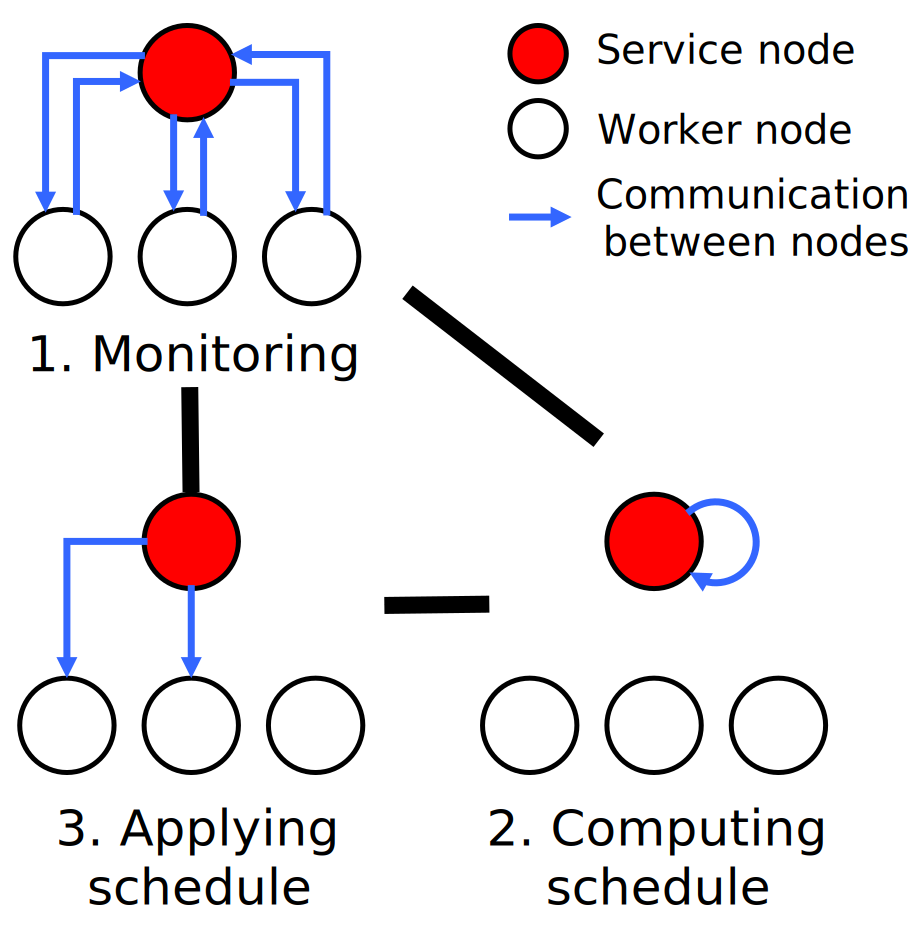
\includegraphics[width=.45\linewidth]{figures/scheduling_steps.pdf}
%         \label{fig:scheduling_steps}}
%         \subfigure[Workload fluctuations during scheduling]{
%         \includegraphics[width=.45\linewidth]{figures/workload_fluctuations2.pdf}
%         \label{fig:workload_fluctuations}}
% \vspace*{-.2cm}
% \caption{VM scheduling in a master/worker architecture}
% \end{center}
% \label{fig:scheduling}
% \vspace*{-.2cm}
% \end{figure}
% %
% \MS[AL]{Must we keep the fig.: the arguments of complexity and time
%   requirements are already made in the remainder of the intro. If we
%   keep it, the discussion should be simplified.}
% Each VMPP mechanism is a complex system that can face
% important side-effects during each of its stages: Monitoring the
% resources usages, computing the schedule and applying the
% reconfiguration (see Figure \ref{fig:scheduling_steps}).
% %
% %
% As an example, a single master architecture can lead, \textit{a priori} to
% important drawbacks. First, during the computation and the application
% of a schedule, a single master cannot take into account new VM
% requirement violations. Second, the time needed to apply a new
% schedule can be particularly important: The longer the reconfiguration
% process, the higher the risk that the schedule may be outdated, due to
% the workload fluctuations, when it is eventually applied (see Figure
% \ref{fig:workload_fluctuations}). Finally, a single master node can
% lead to well-known fault-tolerance issues: A group of VMs may be
% temporarily isolated from the master node in case of a network
% disconnection or if the master node crashes.
% %
Analyzing proposals for VM placement on representative testbeds in
terms of scalability, reliability and varying workload changes would
definitely be the most rigorous way to support their development for
CC production infrastructures.
% and compare  with existing proposals.
However, \textit{in-vivo} experiments, if they can be executed at all,
are always expensive and tedious to perform (see~\cite{barker:pitfalls} for a recent reference).
% They may even be counterproductive if the observed behaviors are clearly
%different from the expected ones.

In this article, we propose \vmps, a dedicated simulation framework to
perform in-depth investigations of VM placement algorithms and compare
them in a fair way. To cope with real conditions such as the
increasing scale of modern data centers, as well as the workload
dynamicity and elasticity characteristics that are specific to the CC
paradigm, \vmps allows users to study large-scale scenarios
%that take into account server crashes and
that involve thousands of VMs,
each executing a specific workload that evolves during the
simulation.
%
%
To illustrate the relevance of \vmps, we have implemented and analyzed
three well-known approaches:
Entropy~\cite{Hermenier:2009:ECM:1508293.1508300},
Snooze~\cite{feller:ccgrid12}, and DVMS~\cite{quesnel:cpe2012}.
% Besides being well-known from the literature,
We chose these three systems as they represent three classes of
placement algorithms: Entropy is an instance of a centralized model,
Snooze of a hierarchical one and DVMS of a fully distributed one.
Using \vmps, we compare the scalability and reactivity (\ie the time
to solve SLA violations) of the strategies --- a contribution of its
own.  Our results also reveal the importance of the duration of the
reconfiguration phase (\ie the step where VMs are relocated throughout
the infrastructure) compared to the computation phase (\ie the step
where the scheduler solves the VMPP).
%
%Built on top of the \sg toolkit~\cite{casanova:hal-01017319},
%
We believe that \vmps will be beneficial to a large number of
researchers in the field of CC as it enables them to analyze the main
characteristics of a new proposal, allowing \textit{in vivo}
experiments to be restricted to placement mechanisms that have the
potential to handle CC production infrastructures.

The rest of the article is
organized as follow.
%Section~\ref{sec:vmpp} highlights the importance of the scalability, reliability and reactivity criterions for the VM
%Placement Problem.
Sec.~\ref{sec:sg} gives an overview of the \sg
framework on which our proposal is built. Sec.~\ref{sec:injector}
introduces \vmps.
% and discusses its general functioning
Entropy, Snooze and DVMS are briefly presented in
Sec.~\ref{sec:vm-schedulers} and evaluated in
Sec.~\ref{sec:experiments}. Secs.~\ref{sec:related}
and~\ref{sec:conclusion} present, respectively, related work and a
conclusion.




%%% Local Variables:
%%% mode: latex
%%% TeX-master: "main"
%%% End:
